\documentclass[a4paper]{article}

\usepackage[utf8]{inputenc}
\usepackage[portuges]{babel}
\usepackage{indentfirst}
\usepackage{graphicx}
\usepackage{float}
\usepackage{caption}
\usepackage{subcaption}
\usepackage[T1]{fontenc}
\usepackage{listings}
\usepackage{amsmath}
\usepackage{mathtools}
\renewcommand{\familydefault}{\sfdefault}


\title{Projeto de Computação Gráfica - Fase 4}
\author{Diogo Braga A82547 \and João Silva A82005 \and Ricardo Caçador A81064
\and Ricardo Veloso A81919}
\date{\today}

\begin{document}

\maketitle

\begin{abstract}
Neste relatório é apresentada a terceira fase dum projeto no qual a intenção é desenvolver um mecanismo baseado em gráficos 3D e fornecer exemplos de uso que mostrem o seu potencial. Este projeto é desenvolvido no âmbito da unidade curricular de Computação Gráfica.
\end{abstract}

\newpage

\tableofcontents


\newpage

\section{Introdução}
\label{sec:intro}

Nesta última fase serão feitas as últimas alterações no \textit{Generator} e no \textit{Engine}.


No caso do \textit{Generator} :

\begin{enumerate}
	\item Serão geradas \textbf{coordenadas} para as texturas.
	\item Serão gerados \textbf{vetores normais} para cada vértice com o objetivo de, posteriormente, proporcionar iluminação.
\end{enumerate}

No caso do \textit{Engine} :

\begin{enumerate}
	\item Realizar o parsing do ficheiro XML que irá conter as informações relativas à ilimunição e às texturas e guardar a informação retirada nas devidas estruturas.
	\item Ativar as funcionalidades da iluminação e das texturas.
	\item Aplicar as \textbf{coordenadas} e os \textbf{vetores criados} no \textit{Generator}.
\end{enumerate}

De seguida iremos apresentar figuras, algoritmos e as suas respetivas explicações de forma a ilustrar a realização das etapas apresentadas acima.

\section{Estrutura da Pasta do Projeto}
\label{sec:estrutura}

Para um entendimento mais claro da estrutura do projeto, achamos por bem referenciar a estrutura da pasta do projeto.
O projeto entregue contêm para além do relatório, 4 pastas como é possível verificar na seguinte figura.

\begin{figure}[H]
\centering
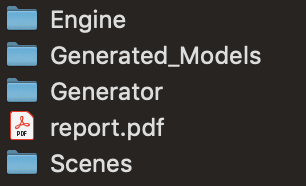
\includegraphics[scale=1.0]{estrutura.png}
\caption{Estrutura da pasta.}
\label{img:estrutura}
\end{figure}

Relativamente à fase anterior não podemos apontar qualquer diferença sendo que não foi acrescentado qualquer ficheiro ou pasta à estrutura do projeto isto porque a quarta e última fase apenas envolve a realização de alterações no código dos ficheiros já existentes.

\newpage

\section{Estruturas de dados}
\label{sec:estruturadados}

No que conta a estruturas de dados há alguns aspetos importantes a abordar.

Para a iluminação foram criadas duas novas estruturas: \textbf{Color} e \textbf{Light}.



\section{Iluminação}
\label{sec:iluminacao}

\subsection{Parser XML}
\label{sec:parseri}

\subsubsection{Ficheiro}
\label{sec:ficheiroi}

\subsubsection{Funcionamento}
\label{sec:funcionamentoi}

\subsection{Engine}
\label{sec:enginei}

\subsection{Generator}
\label{sec:generatori}

\section{Texturas}
\label{sec:texturas}

\subsection{Parser XML}
\label{sec:parsert}

\subsubsection{Ficheiro}
\label{sec:ficheirot}

\subsubsection{Funcionamento}
\label{sec:funcionamentot}

\subsection{Engine}
\label{sec:enginet}

\subsection{Generator}
\label{sec:generatort}

\section{Conclusão}
\label{sec:conclusao}

\end{document}